\section{Results}\label{sec:results}
In this section we investigate the how parallelisms affected our program. We
break the report into three sections. In the first section (Sec~\ref{sec:r-opt})
we discuss the optimization techniques we performed, in the second
section (Sec~\ref{sec:r-omp}) we discuss our OpenMP implementation, and finally
in the third section (Sec~\ref{sec:r-cuda}) we discuss our CUDA implementation. 

\subsection{Serial Optimizaton}\label{sec:r-opt}
In common fashion, before we start implementing parallelization we first started
optimizing the serial implementation of our code. We do this first because many
optimization techniques are about memory access and reducing the number of times
an address is accessed. This helps with both OpenMP and CUDA parallelization
because in both cases we will still want to reduce our memory footprint. While
CUDA optimization won't see as much benefits from this exercise, as CUDA
optimization is more dependent upon multi-dimensional memory access, using
blocks and grids, it will still be beneficial overall. 

To do this first took our working code and profiled it. Because our code allows
for arbitrary sized neural networks we increased the number of hidden layers and
neurons to get better profiling, though this decreased our accuracy. 
%We
%increased to 5 hidden layers (7 total) and each hidden layer had 300 neurons.
%This was a fair balance between taking too long to compute and not having enough
%work to perform. 
Profiling the code this way we looked for areas where we could
first pre-allocate memory, This had significant effects in the speedup. We then
looked for loops where we could reduce redundant computation, for example
calculating the vector size every loop iteration. An example of this shown in 
Figure~\ref{fig:opt}. These types of optimizations significantly improved our
results. 

\begin{figure}[ht]
(a)
\begin{lstlisting}[language=C++,
                   directivestyle={\color{black}},
                   emph={size_t},
                   emphstyle={\color{blue}}]
for(size_t i = 0; i < v.size(); ++i)
 for(size_t j = 0; j < v[0].size(); ++j)
  computation
\end{lstlisting}
(b)
\begin{lstlisting}[language=C++,
                   directivestyle={\color{black}},
                   emph={size_t},
                   emphstyle={\color{blue}}]
size_t v_size = v.size();
size_t v0_size = v[0].size();
for(size_t i = 0; i < v_size; ++i)
 for(size_t j = 0; j < v0_size; ++j)
  computation
\end{lstlisting}
\caption{Reducing loop lookups. (a) unoptimized (b) optimized}
\label{fig:opt}
\end{figure}

Previous to these, and other, optimizations our functions were not near the
worst performers according to $gprof$. After these we had our matrix multiply
function, our transpose, and our vector addition near the top. All these
optimizations ensured that there was proper pipelining and that we could fully
exploit our parallelism. One final optimization that we did is optimize the
matrix multiplication to get the best indexing we could, over a naive version
that was initially implemented. This provided the largest speedup.

\subsection{OpenMP Implementation}\label{sec:r-omp} 

After we have ensured that proper pipelining and serial optimization are
implemented the next task is to parallelize. Because of the shared memory in
OpenMP our optimizations in Section~\ref{sec:r-opt} we only have to access these
memory points once and then we can share that memory across the threads. Because
most of our computation was in the form of vector or matrix operations we can
pipeline like above, share the memory, and parallelize the outer most loop so
that we can exploit the faster stride on the inside of the loop, since those
points are contiguous in memory and the outer loop isn't. 

To parallelize our code we focused on our math library, which held all our
mathematical functions and performs all our tensor operations. We investigated
parallelizing every operation and found that most operations had little to no
effect. A major hurdle we had was that we found that we needed hundreds of
neurons and a fair amount of layers for parallelism to create several hidden
layers. For the problems we are solving, such as the half moon, this is far too
large to learn the dataset and will over fit. For example, to learn the half
moon dataset we only needed 2 input neurons, a single hidden layer with 3 neurons,
and an output layer. With this network, not even a ``deep'' neural network,
we quickly converged on the answer, typically below 100 epochs. The
parallelization helps significantly more when increasing the number of neurons
as opposed to the depth of the network, or the number of hidden layers. But
since our goal was to build a framework, similar to PyTorch, we just needed to
test the parallelization rather than solve a specific problem. Thus we created
experiments with 300 neurons in each hidden layer and 5 hidden layers. We found
this to be a good balance between the program not taking too long to run and
having enough work to see speedups from parallelism. 

To see the effect of parallelism we perform a small ablation study to see what
was needed for speedup and what wasn't. We show the results of this in
Figure~\ref{fig:omp}. As we can see here, the matrix multiply parallelization
had the largest impact on speedup. Without this the other cases actually
increase as the number of CPUs increase. Note that we are parallelizing most
functions and these do have some overhead. Interestingly we find that the run
without either matrix multiply nor vector add implemented runs slightly faster
than when just matrix multiply is removed. We believe that this is because of
the lack of work. One other factor to note is that at 16 threads we note a
slight increase, where previously we were strictly decreasing. This is because
our machine has 16 physical cores 16 but they have 2 threads per core. Some work
performs better on physical cores rather than hyper-threading, which is why it
is turned off in many HPC applications, and we see that this holds true here. To
aid in this analysis we draw a vertical gray line to bifurcate where
hyper-threading begins. We
note that our fastest run was at 16 threads, executing at $40.128$s ($4.47$x
speedup) and the 32 thread implementation ran at $46.072$s ($3.89$x speedup). We
also note that the fastest hyper-threading implementation happened at 28
threads, $42.938$s ($4.17$x speedup). We believe that this is due to some
peculiarity in how hyper-threading works. We notice that there was more
uncertainty within this region. This gives evidence that for faster and more
stable computation one should disable hyper-threading.

\begin{figure}[ht]
\centering
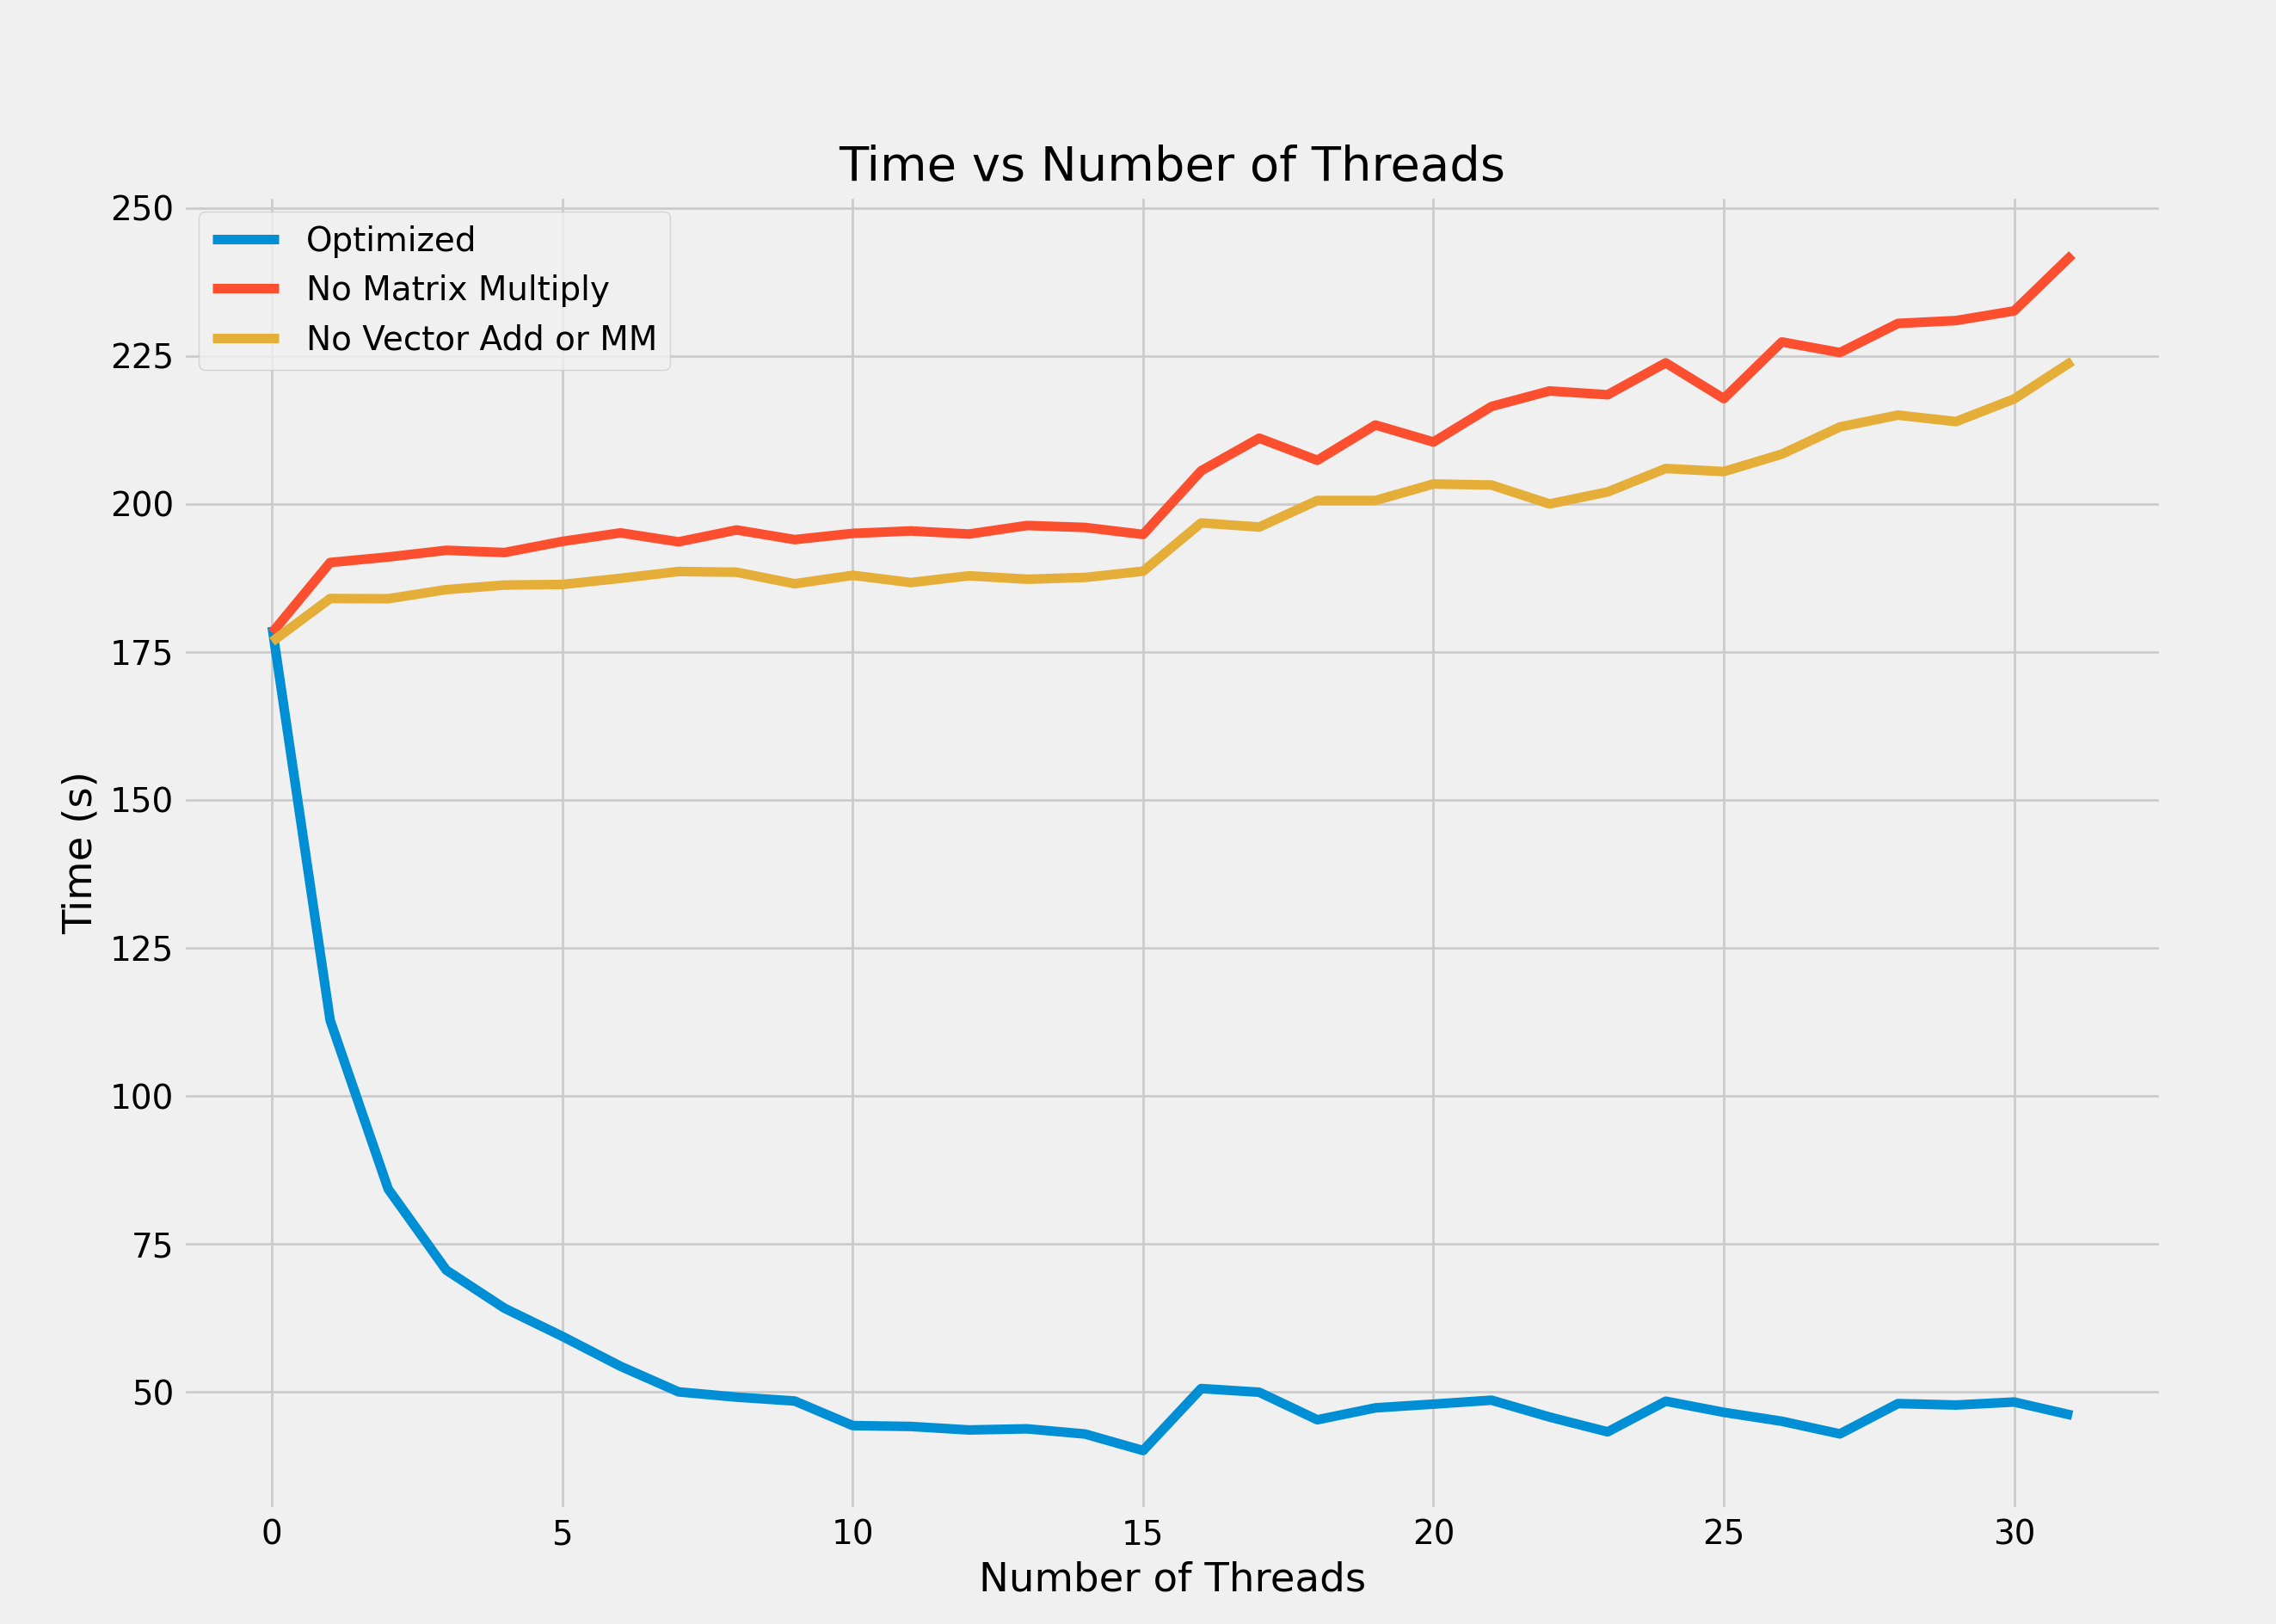
\includegraphics[width=\linewidth]{omp.png}
\caption{Comparison of how different functions affect parallelization results,
    using OpenMP}
    \label{fig:omp}
\end{figure}

Additionally we look at our matrix multiplication vs using a cache optimized
version. To create our cache optimized matrix we divide our i,j, and k indices
into smaller blocks. This allows for the multiplication to be better localized
in memory. We can see the results in Figure~\ref{fig:mm}. Here we see that our
cache efficient matrix multiply actually receives better performance increase
under initial parallelization, achieving roughly a $14.5$x speedup at 5 threads,
while our naive implementation only achieves a $4.5$x speedup at best. This
suggests that the blocking version of matrix multiply could potentially be more
efficient but that we do not have sufficient workloads to benefit from this type
of parallelization. We would expect this version to be more efficient because it
is more cache efficient. Unfortunately, in our workload we have matrices where
the number of rows is far larger than the number of columns, often as small as
2, and that causes more cache misses than hits. Even worse, in our
implementation many times we have vectors be multiplied and thus we do not gain
any benefit at all. This type of multiplication has much larger overhead and we
would not expect it to perform better than the naive version unless we were
dealing with substantially larger matrices where we had issues fitting a row of
data into memory. Interestingly in the cache efficient version we see that the
computation diverges upon evoking hyper-threading as well as becomes less
stable. We believe that hyper-threading suffers much harsher penalties to cache
misses than physical cores do and that this causes the divergent behavior. We
predict that if we were learning on larger datasets, such as ImageNet, we would
see better performance increases from these type of optimizations. 

% We see here that we
% don't get speedup even though we are better cache aligned. The reason, again,
% for this is because the lack of work as well as the size of the matrices. The
% problem with this is that our matrices aren't very large. Which we have many
% rows, we don't have very many columns. This causes no real speedup from blocking
% the matrices up because at most we can block is 2. This ends up causing more
% cache misses than hits. We predict that even MNIST wouldn't give us a
% significant improvement. We do not expect this to provide significant speedups
% until we start working on larger problems like ImageNet. Additionally we had
% problems with the block matrices because our matrices were inconsistent sizes,
% including sometimes vectors. Vectors happened when at the final layer. This made
% for very inconsistent results. We got the best results when blocking by 2 and
% checking if our matrix sizes were even first. 

\begin{figure}[ht]
\centering
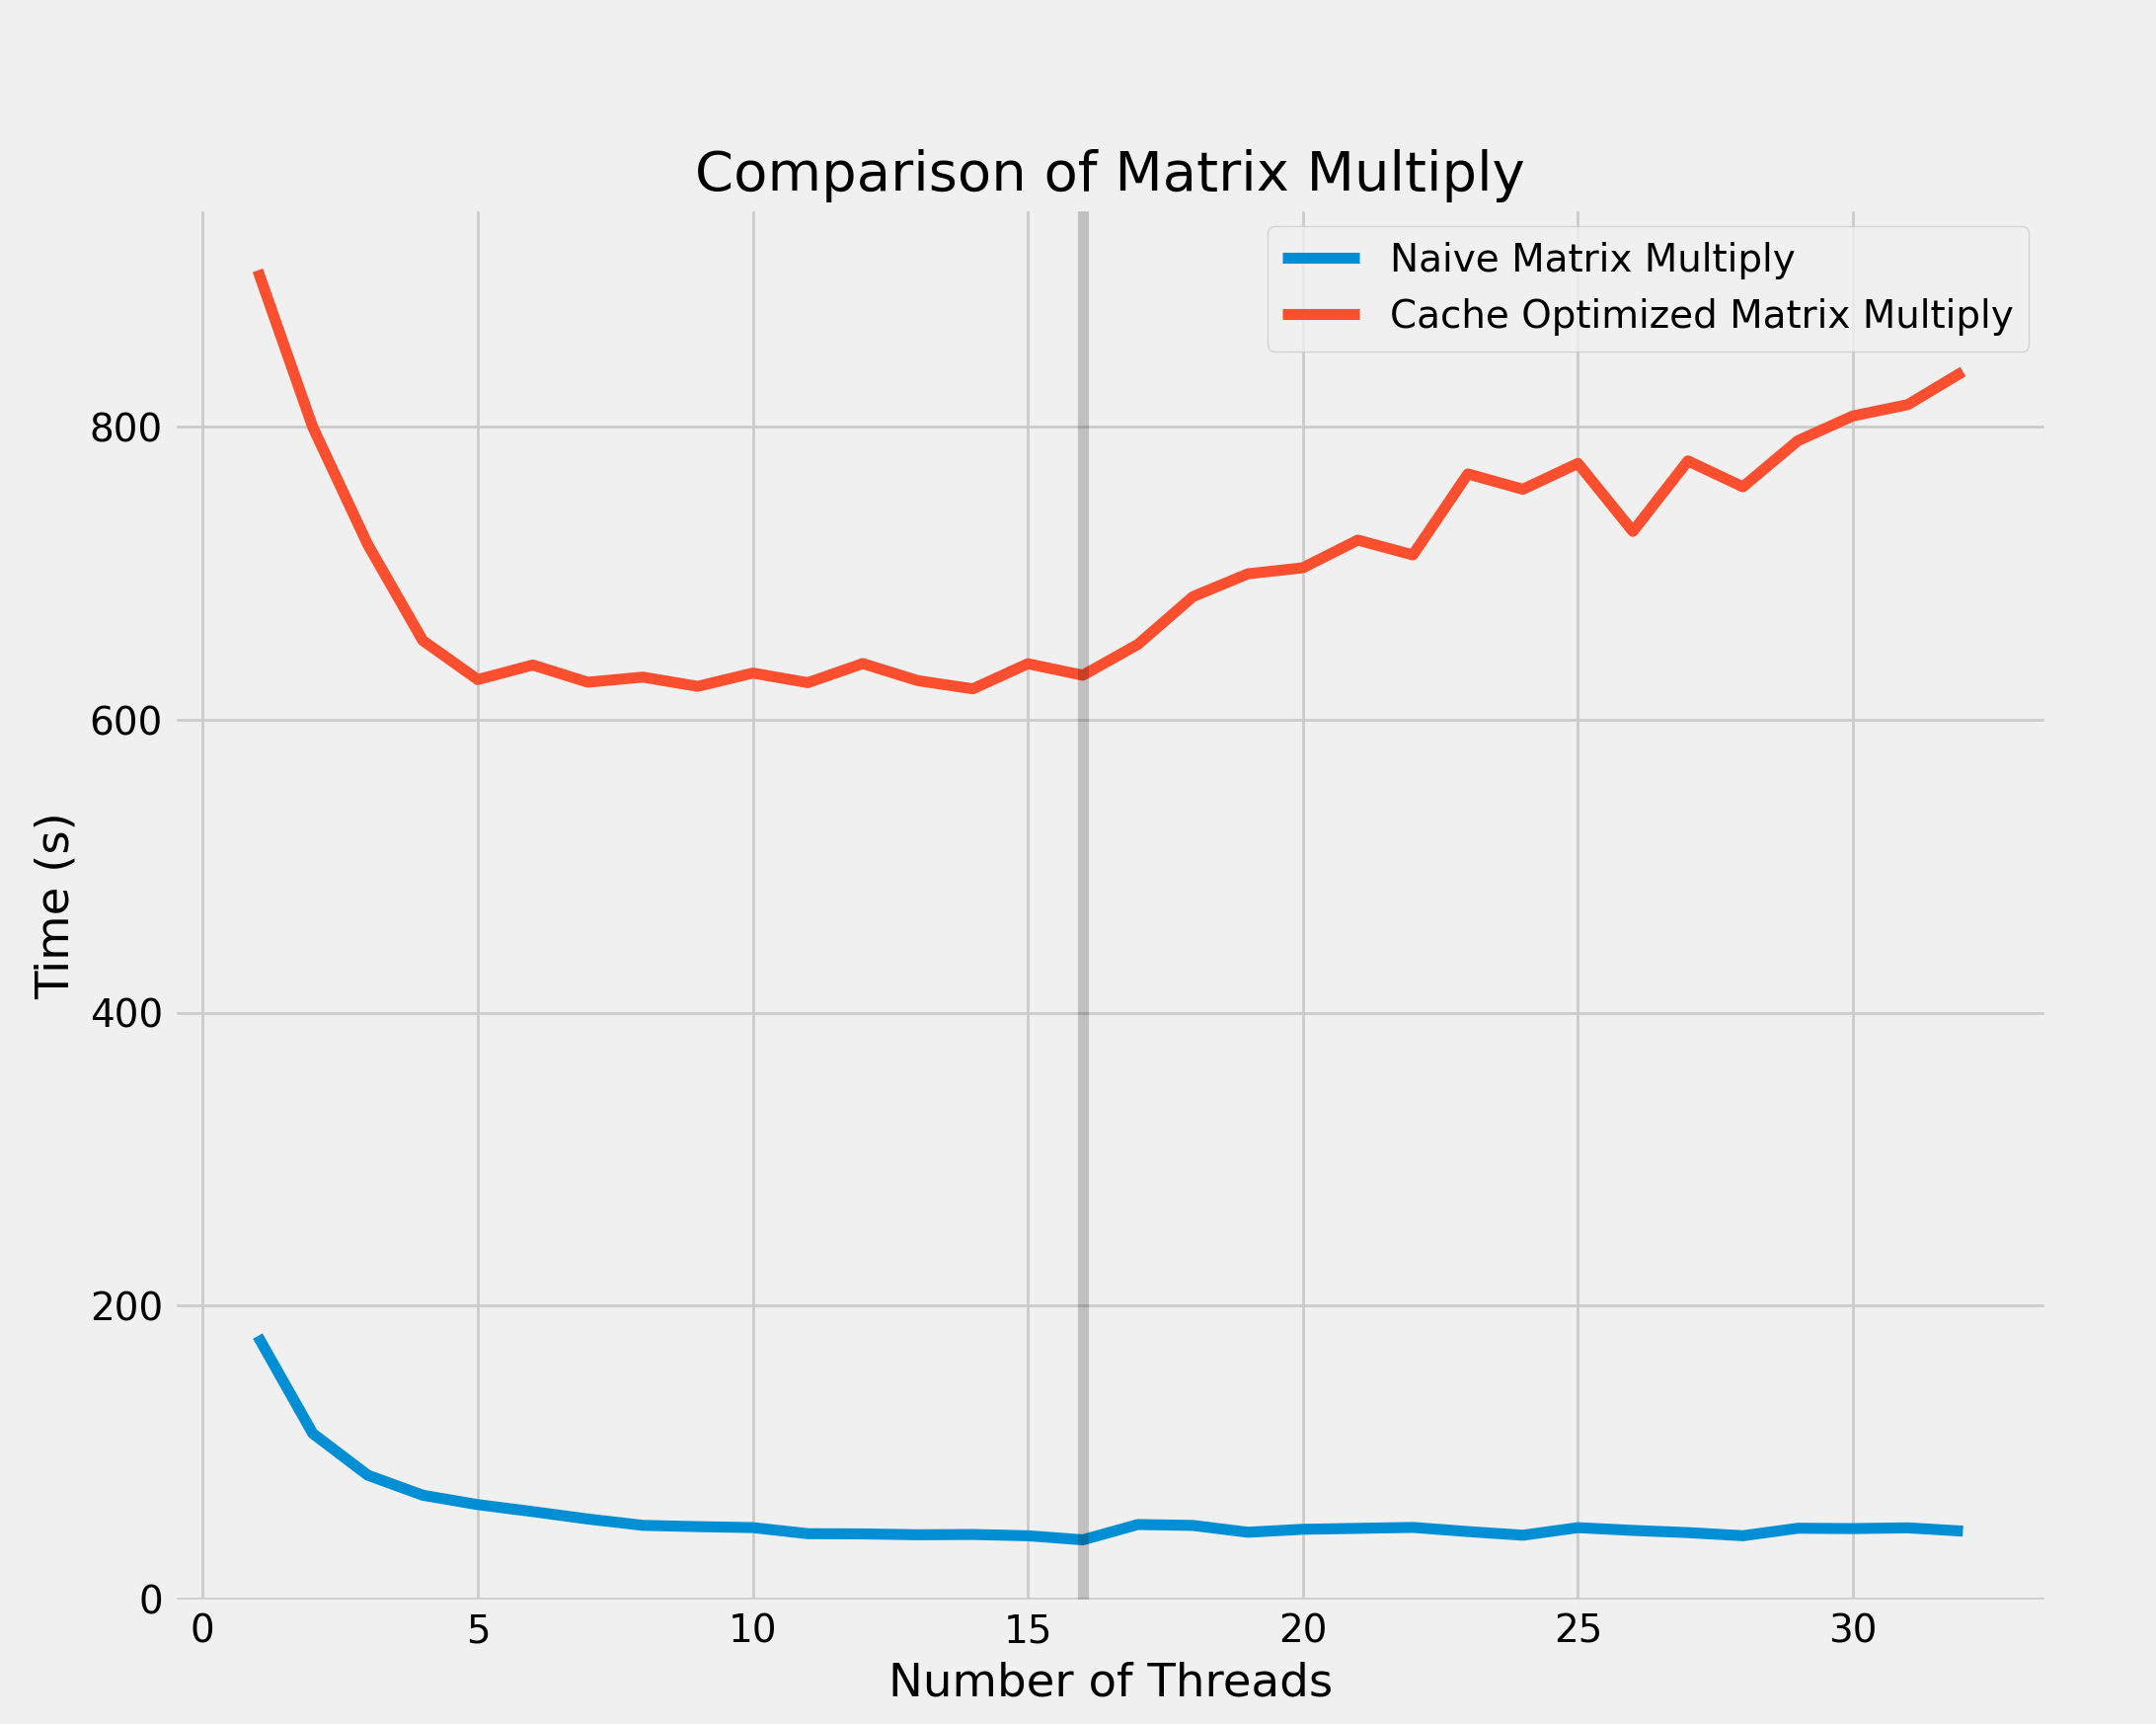
\includegraphics[width=\linewidth]{mm.png}
\caption{Comparison of different Matrix Multiply methods}
    \label{fig:mm}
\end{figure}

\subsection{CUDA}\label{sec:r-cuda}
We were unfortunately unable to get the entire model into CUDA but we still
wanted to provide some motivation as to how GPU acceleration would help with our
problem. Knowing that PyTorch and TensorFlow benefit a lot from GPU acceleration
we investigated how performing our matrix multiplication and transpose functions
would help. For similar reasons as in the OpenMP example we didn't implement a
block matrix setup in CUDA, and actually struggled with trying to implement
this. The same is true for the efficient matrix transpose. Instead we just kept
the naive algorithms. To make a fair comparison we timed our results in two
different ways. The first we did was timing the matrix multiple with the
communication time and we also timed just the kernel execution. We figured that
testing the kernel function would give us a good indication of how fast a fully
GPU implementation would run compared to the CPU version. Unfortunately we found
that we were still slower in the GPU implementation. While our OpenMP solution ran
in $1.213\mu s$ our CUDA kernel function ran in about $4.98\mu s$ and including
communication time $121.734\mu s$.

Our working theory of why we are not seeing improvements with GPU acceleration
is two fold. We believe that the largest contributor to our problem is actually
the problem type. Because we are trying a simple classification we have matrices
where $m>>n$. The optimized matrix multiplications do not perform well in these
shaped matrices, performing best in square like matrices. The second issue is
that the work itself isn't very large, only having 300 neurons per layer. We saw
similar relationships with around 1000 neurons per layer, testing with a small
number of epochs, but did not record the times because we could not do a full
run in a reasonable amount of time. Linear layers of this size are also atypical
in modern networks so we decided it was not a good avenue to pursue. 

